Tässä luvussa esitetään tutkimuksen tärkein sisältö ja kokonaisuutena vastaus tutkimuskysymykseen \emph{T1}, eli toistettavissa oleva menetelmä testitapauksien priorisoimiseen.
Priorisointiin vaikuttavat muuttujat luvussa \ref{ch:10_priorisointiin_vaikuttavat_muuttujat} esitetään myös suora vastaus tutkimuskysymykseen \emph{T2}.
Lisäksi painofunktiot \ref{ch:10_painofunktiot_priorisointiin} ja verkon karsiminen \ref{ch:10_verkon_karsiminen} esittää vastaukset tutkimuskysymykseen \emph{T3}.
Testitapauksien muodostaminen verkosta \ref{ch:10_testitapauksien_muodostaminen_verkosta} antaa osittaisen vastauksen myös tutkimuskysymykseen \emph{T4}.

Priorisointia varten esitetään harkintaa käyttäen valitut priorisointiin vaikuttavat muuttujat, niitä käyttävät painofunktiot, verkon rakentaminen ja karsiminen sekä verkon ja testitapauksien yhteys.
Lisäksi menetelmää käyttäen tuotetun painotetun verkon sisältämää informaatiota käytetään prioriteeteiltaan tärkeimmän polun löytämiseen.

\section{Priorisointiin vaikuttavat muuttujat} \label{ch:10_priorisointiin_vaikuttavat_muuttujat}

  Näkymä- ja siirtymäperustaiseen priorisointiin vaikuttavat monet eri asiat, joista osa kasvattaa prioriteettia ja osa laskee sitä.
  Prioriteettia kasvattava muuttuja on esimerkiksi liiketoiminnallinen arvo ja laskeva muuttuja on esimerkiksi projektin muutosherkkyys.
  Muuttujat ovat kuitenkin hyvin kontekstiriippuvaisia, joten yleispätevää ja kaikkiin tilanteisiin soveltuvaa listaa muuttujista on hankala antaa.
  Kontekstiriippuvaisuuden takia muuttujiin ja myöhemmin esitettäviin painofunktioihin on varattu paikka omille lisämuuttujille.

  Tässä diplomityössä esiteltävää priorisointimenetelmää varten jokainen priorisointiin vaikuttava muuttuja arvioidaan asteikolla 1-10, paria poikkeusta lukuun ottamatta.
  Numeerisella asteikolla on tarkoitus antaa korkea numero, jos muuttuja on prioriteetiltaan tärkeä kyseisen näkymän, eli verkon solmun kohdalla.
  Jos jokin muuttuja ei ole kelpoinen siinä kontekstissa, jossa menetelmää yritetään hyödyntää, tulee muuttujan arvo asettaa nollaksi, jolloin se sivuutetaan painofunktiossa \ref{ch:10_painofunktiot_priorisointiin}.

  Poikkeukselliset muuttujat ovat käyttötapauksien määrä ja siirtymien määrä, joissa numeerisen asteikon sijaan käytetään kyseisten muuttujien määrää suhteessa koko verkkoon.
  Esimerkiksi siirtymien määrää ilmaiseva suhde määritetään laskemalla solmun asteluku \(d_G(v)\), eli solmuun liittyneiden kaarien määrä, jaettuna kaikilla verkossa olevien kaarien määrällä.
  Lisäksi siirtymien määrän suhde vielä kerrotaan luvulla 10, jotta se saadaan skaalautumaan muiden muuttujien kanssa samalle tasolle.

  \begin{table}[H]
    \caption{Priorisointiin vaikuttavat muuttujat}
    \label{tab:priorisointiin_vaikuttavat_muuttujat}
    \centering
    \begin{tabular}{lllll} \hline
    \(m\) & \textbf{Muuttuja} & \textbf{Etumerkki} & \textbf{Asteikko} &  \\ \hline
    \textbf{1} & Liiketoiminnallinen arvo & \(+\) & 1 - 10 &  \\
    \textbf{2} & Liiketoiminnallinen visio & \(+\) & 1 - 10 &  \\
    \textbf{3} & Negatiivinen käyttäjäpalaute & \(+\) & 1 - 5 &  \\
    \textbf{4} & Käyttötapauksien määrä & \(+\) & 10 \(\cdot\) suhde &  \\
    \textbf{5} & Siirtymien määrä & \(+\) & 10 \(\cdot\) suhde &  \\
    \textbf{6} & Positiivinen käyttäjäpalaute & \(-\) & 1 - 5 &  \\
    \textbf{7} & Muutosherkkyys & \(-\) & 1 - 10 &  \\
    \textbf{8} & Toteuttamisen kompleksisuus & \(-\) & 1 - 5 &  \\
    \textbf{9} & Toteutuksen virheherkkyys & \(-\) & 1 - 5 &  \\
    \textbf{10} & Omat lisämuuttujat & \(\pm\) & 1 - 10 & \\ \hline
    \end{tabular}
  \end{table}

\section{Painofunktiot priorisointiin} \label{ch:10_painofunktiot_priorisointiin}

  Painofunktioiden määrittäminen on tärkeä osa painotetun verkon avulla priorisointia, sillä niiden avulla määritetään verkon solmujen ja kaarien prioriteetit.
  Tavanomaisesti numeerinen prioriteetti usein mielletään olevan korkea, jos priorisoitu muuttuja on tärkeä.
  Painotettujen verkkojen tapauksessa on kuitenkin järkevää vaihtaa numeerisen prioriteetin suuntaa, jotta painotettuun verkoon sovellettavat lyhimmän polun algoritmit toimisivat etsien prioriteetiltaan tärkeitä polkuja. Ennen prioriteetin suunnanvaihtoa, voidaan kokonaisprioriteetti \(p\) yksittäiselle solmulle \(v\), eli näkymälle määrittää seuraavasti.

  \[p(v) = \sum\limits_{i=1}^{5} m_i - \sum\limits_{j=6}^{9} m_j \pm m_{10}\]

  Prioriteetin suunnan vaihtamiseksi suuresta pieneen, säilyttäen kuitenkin prioriteetin sisältämän informaation, voi hoitaa käänteislukujen avulla.
  Ennen käänteisluvuksi muuttamista, prioriteettiin vaikuttavien muuttujien yhteenlaskettu summa voi olla ongelmallisesti negatiivinen tai nolla.
  Negatiiviset arvot eivät ole painotetun verkon kannalta erityisen järkeviä, sillä tässä diplomityössä hyödynnettävää Dijkstran algoritmia ei voida käyttää negatiivisien painojen kanssa.
  Dijkstran algoritmin toiminta nollan tapauksessa voi myös kuulostaa epäilyttävältä, kuten esimerkiksi tilanne, jossa painotetun verkon kaikki painot olisivat nollia.
  Dijkstran algoritmin tapauksessa tällainen verkko on kuitenkin sallittu, koska silloin lyhimmän polun ratkaisu on verkon kaikki solmut.
  Lyhimmän polun ongelman erityisvaatimusten lisäksi käänteislukua varten nolla on huono arvo siinä mielessä, että sille ei ole olemassa lainkaan käänteislukua.
  Tämä johtuu siitä, että jos nollalle yrittäisi etsiä käänteislukua, tulisi eteen nollalla jakaminen jota ei voi tehdä.
  Nämä molemmat ongelmatapaukset voidaan kuitenkin painofunktiossa ratkaista siten, että käänteisfunktiota ei etsitä, vaan korvataan painofunktion tulos yhdellä.

  Painofunktio yksittäiselle solmulle \(v\), eli näkymälle saadaan solmun kokonaisprioriteetin \(p(v)\) käänteislukuna.

  \[\alpha(v) = \begin{cases}
    p^{-1}(v) & p(v) > 0 \\
    1 & p(v) \leq 0
  \end{cases}\]

  Painofunktio yksittäiselle solmut \(v_x\) ja \(v_y\) yhdistävälle kaarelle \(e_{xy}\), eli siirtymälle saadan myös käänteislukuna.
  Kaaren painofunktiota varten pitää kuitenkin huomioida, että sen kokonaisprioriteetti on kaaren solmujen kokonaisprioriteetin summa \(p(v_x) + p(v_y)\).
  Kaaren kokonaisprioriteetti \(p(v_1) + p(v_2)\) pitää laskea ennen käänteisluvuksi muuttamista.

  \[\beta(e_{xy}) = \begin{cases}
    (p(v_x) + p(v_y))^{-1} & p(v_x) + p(v_y) > 0 \\
    1 & p(v_x) + p(v_y) \leq 0
  \end{cases}\]

\section{Verkon rakentaminen} \label{ch:10_verkon_rakentaminen}

  % TODO: Miten verkon solmut ja kaaret poimitaan käyttöliittymästä ja taulukon esittely
  \begin{itemize}
    \item <TODO: Kirjoita teksti miten verkon solmut ja kaaret poimitaan käyttöliittymästä>
  \end{itemize}

  \begin{table}[H]
    \caption{Esimerkkiverkon näkymät, siirtymät ja priorisointimuuttujat}
    \label{tab:esimerkki_verkon_priorisointi_muuttujat}
    \centering
    \begin{tabular}{lllllllllllll} \hline
    \(n\) & \textbf{Näkymä} & \textbf{Siirtymät} & \(m_1\) & \(m_2\) & \(m_3\) & \(m_4\) & \(m_5\) & \(m_6\) & \(m_7\) & \(m_8\) & \(m_9\) & \(p(n)\) \\ \hline
    \textbf{A} & Kirjautuminen & B & 10 & 10 & 0 & 2 & 1 & 0 & 5 & 5 & 5 & 8 \\
    \textbf{B} & Pelivalikko & A, C, D, G & 8 & 10 & 1 & 2 & 4 & 4 & 5 & 5 & 5 & 6 \\
    \textbf{C} & Asetukset & A, B & 4 & 6 & 5 & 2 & 2 & 2 & 5 & 5 & 5 & 2 \\
    \textbf{D} & Peli & B, E, G & 10 & 10 & 4 & 2 & 3 & 4 & 4 & 5 & 5 & 11 \\
    \textbf{E} & Tulokset & B, D, F & 6 & 8 & 0 & 2 & 3 & 5 & 5 & 4 & 5 & 2 \\
    \textbf{F} & Onnittelu & B, E & 1 & 8 & 0 & 0 & 2 & 2 & 5 & 2 & 5 & -3 \\
    \textbf{G} & Ohje & B, D & 1 & 10 & 2 & 0 & 2 & 0 & 8 & 0 & 0 & 7 \\ \hline
    \end{tabular}
  \end{table}

  % TODO: Päivitä painomatriisi vastaamaan esimerkkiä
  \begin{itemize}
    \item <TODO: Kirjoita teksti esimerkkille painomatriisista, jota käytetään priorisoinnin syötteenä>
  \end{itemize}

  Painomatriisin painot on laskettu käyttäen aiemmin esitettyjä painofunktioita \(\alpha\) ja \(\beta\).

  \[\beta(e_{AB}) = (p(v_A) + p(v_B))^{-1} = (8 + 6)^{-1} = \frac{1}{14} \approx 0.071\]

  \[
    M_G \approx
    \bordermatrix{
      G & v_A & v_B & v_C & v_D & v_E & v_F & v_G \cr
      v_A & \infty & 0.071 & 0.100 & 0.053 & 0.100 & 0.200 & 0.067 \cr
      v_B & 0.071 & \infty & 0.125 & 0.059 & 0.125 & 0.333 & 1.000 \cr
      v_C & 0.100 & 0.125 & \infty & 0.077 & 0.250 & 1.000 & 0.111 \cr
      v_D & 0.053 & 0.059 & 0.077 & \infty & 0.077 & 0.125 & 0.250 \cr
      v_E & 0.100 & 0.125 & 0.250 & 0.077 & \infty & 1.000 & 0.111 \cr
      v_F & 0.200 & 0.333 & 1.000 & 0.125 & 1.000 & \infty & 0.250 \cr
      v_G & 0.067 & 1.000 & 0.111 & 0.250 & 0.111 & 0.250 & \infty \cr
    }
  \]

  % TODO: Päivitä kuva vastaamaan esimerkkiä
  \begin{itemize}
    \item <TODO: Kirjoita teksti esimerkille painotetusta verkosta, jota käytetään priorisoinnin syötteenä>
    \item <TODO: Kirjoita teksti, että painomatriisin lisäksi jokaiselle solmulle annetaan \(\alpha(v)\) mukainen paino lopulliseen graafiin>
  \end{itemize}

  \begin{figure}[H]
    \centering
    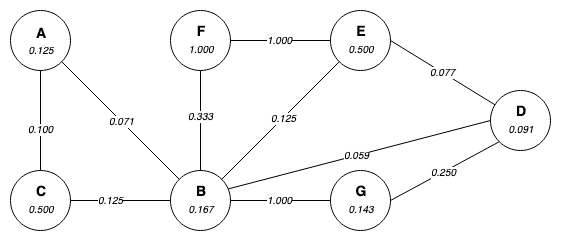
\includegraphics[width=0.6\textwidth]{assets/painotettu-verkko-ennen.png}
    \caption{Esimerkki painotetusta verkosta ennen leikkauksia}
    \label{fig:painotettu-verkko-ennen}
  \end{figure}

\section{Verkon karsiminen} \label{ch:10_verkon_karsiminen}

  Painotetun verkon karsiminen eli leikkaaminen on prioriteeillä painotetun verkon tärkeä ominaisuus.
  Verkkoteorian soveltaminen prioriteettien avulla painotettuun verkkoon on erityisen hyödyllistä, kun verkon kaarissa alhainen paino tarkoittaa suurta prioriteettia.
  Verkon karsimista varten valitaan kattavuus, joka vastaa minimirajaa ja jonka jälkeen karsiminen lopetetaan.
  Kattavuus tarkoittaa myös testikattavuutta testikokoelmien näkökulmasta, sillä painotetussa verkossa jokainen solmu, eli näkymä vastaa näkymän mukaan kategorisoitua testikokoelmaa.

  Verkkoon tehtäviä leikkauksia varten tarvitsee määrittää haluttu kattavuus \(0 \leq c \leq 100\), joka on prosentuaalinen luku siitä kuinka suuri osa verkon solmuista eli näkymistä tai testikokoelmista täytyy verkkoon jäädä karsimisen jälkeenkin. Leikkauksien tekeminen ja toistaminen suoritetaan käyttäen seuraavia toimenpiteitä \(n\)-kertaa, niin kauan kunnes karsittu aliverkko on suurempi kuin kattavuuden mukaan laskettu osuus alkuperäisestä verkosta tai jos iteraatiokerralla ei enää löydy toimenpiteillä poistettavia solmuja.
  \[|V(G_s)| > c \cdot \frac{|V(G)|}{100}, G_s \subset G\]

  Tässä verkon karsimisen esimerkissä kattavuutena käytetään \(c = 80\), joka tarkoittaa esimerkin solmujen määrän \(7\) karsimista \(80 \cdot \frac{7}{100} = 5.6\), eli lukumäärään \(5\) asti.

  \begin{enumerate}
    \item Poistetaan verkosta löytyvä eristetty solmu, eli solmu jonka asteluku on nolla.
    \[d_G(v) = 0\]
    \item Poistetaan verkosta löytyvä sillattu solmu, eli solmu jonka asteluku on yksi ja paino on pienempi kuin solmujen painojen keskiarvo.
    \[d_G(v) = 1  \land \alpha(v) > \frac{1}{|V(G)|} \cdot \sum\limits_{v \in V(G)} \alpha(v)\]
    \item Poistetaan verkosta sellainen alhaisimman prioriteetin solmu, jonka asteluku on pienempi kuin solmujen astelukujen keskiarvo ja paino on pienempi kuin solmujen painojen keskiarvo.
    \[d_G(v) < max\{d_G(x) | x \in V(G)\} \land \alpha(v) > \frac{1}{|V(G)|} \cdot \sum\limits_{v \in V(G)} \alpha(v)\]
  \end{enumerate}

  % TODO: Päivitä kuva vastaamaan esimerkkiä
  \begin{figure}[H]
    \centering
    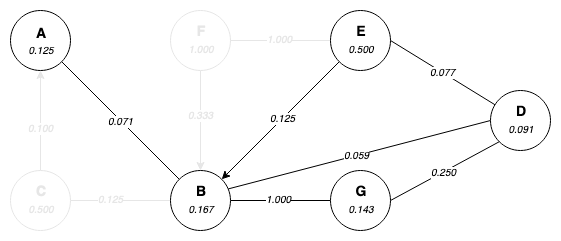
\includegraphics[width=0.6\textwidth]{assets/painotettu-verkko-jalkeen.png}
    \caption{Esimerkki painotetusta verkosta leikkauksien jälkeen}
    \label{fig:painotettu-verkko-jalkeen}
  \end{figure}

\section{Dijkstran algoritmin hyödyntäminen} \label{ch:10_dijkstran_algoritmin_hyodyntaminen}

  Priorisointimenetelmän mukaan karsittuun painotettuun verkkoon on mahdollista soveltaa lyhimmän polun ongelman ratkaisemiseen kehitettyjä algoritmeja, jolloin ne toimivat etsien alhaisimman, eli korkeimman prioriteetin polkuja.
  Lyhimmän polun etsimiseen on tarkoituksenmukaista valita aina aloitus ja lopetuspisteet, joiden välille lyhin polku verkossa voidaan etsiä.
  Prioriteetein painotetun verkon tärkeimpien solmujen selvittämistä varten olisi järkevää valita sellaiset aloitus- ja lopetuspisteet, joiden välillä ei näyttäisi olevan korkean painon, eli alhaisen prioriteetin solmuja.

  \begin{itemize}
    \item <TODO: Valitaan min v1 ja v2 ja käytetään dijkstran algoritmia niille>
  \end{itemize}

\section{Verkon ja testitapauksien yhteys} \label{ch:10_verkon_ja_testitapauksien_yhteys}

  Ennen testitapauksien suunnittelua tehtävä priorisointi kuvainnollistaa käyttöliittymän näkymiä, niiden osanäkymiä ja niiden välisiä siirtymiä.
  Tällaisesta painotetusta verkosta saadaan priorisoitua näkymät ja siirtymät, mutta lopulliset testitapauksien prioriteetit ovat testitapaukseen kuuluvien näkymien tai siirtymien prioriteetteja.
  Tämä tarkoittaa käytännössä sitä, että kun näkymät ja siirtymät on priorisoitu, on esimerkiksi yhden yksittäisen tarkasteltavana olevan näkymän toiminnoilla sama keskenään prioriteetti.
